\section{Hardware}

Board components are annotated in \Fref{fig:board}.  A detailed mechanical drawing describing the board dimensions and locations of key components is available on the \productWebPage{}.

\vskip 2em

\begin{figure}[H]
    \centering
    \begin{tikzpicture}[annotation/.style={circle, draw=black, fill=white, very thick, minimum size=7mm}]
        \node at (0,0) {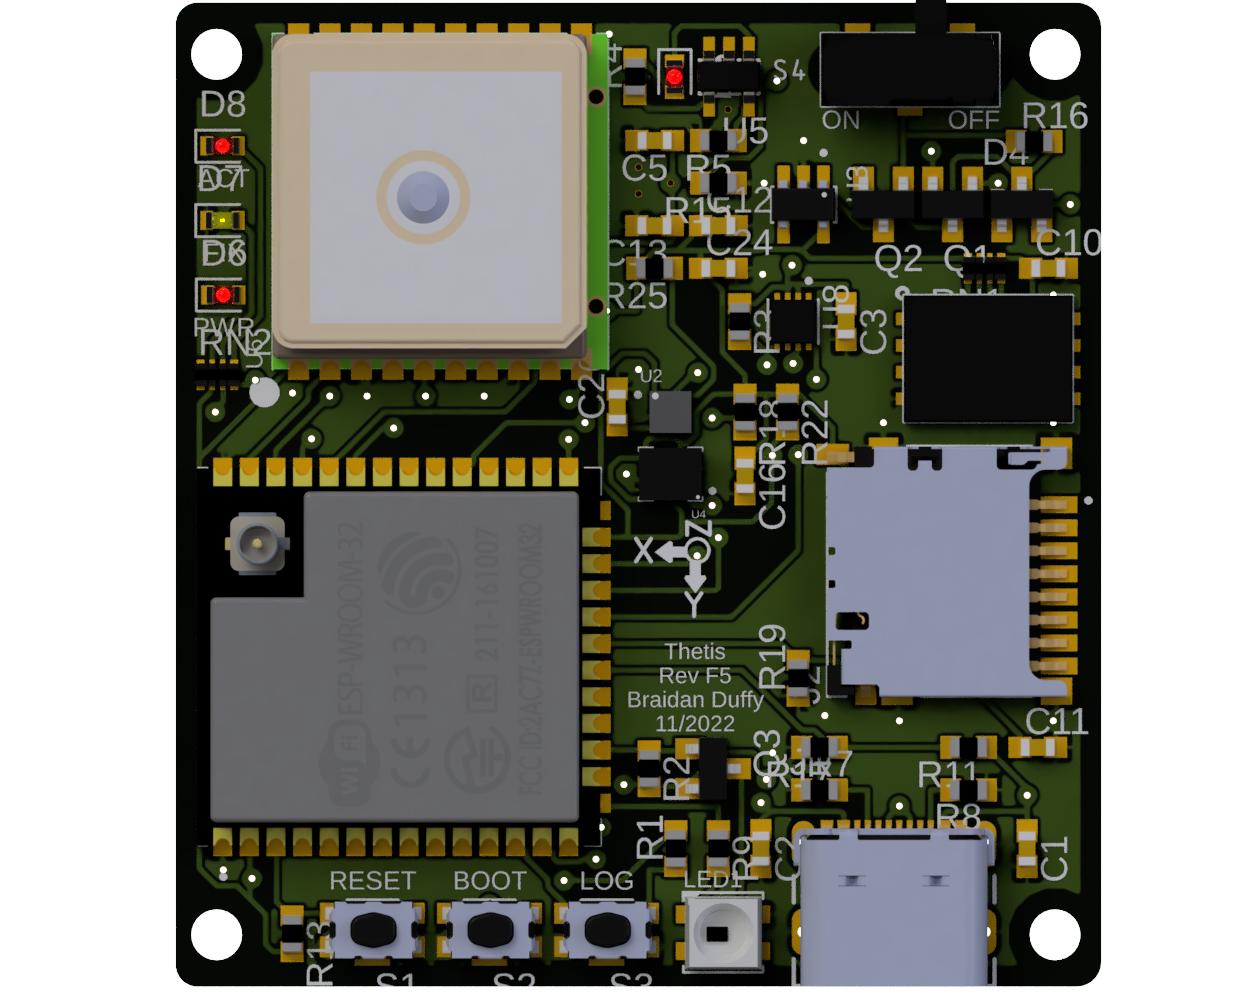
\includegraphics[width=0.95\textwidth]{Images/board.png}};
        \node[annotation] at (-6,-4) {\ref{itm:1}};
        \node[annotation] at (-6.5,0) {\ref{itm:2}};
        \node[annotation] at (-5.7,3.7) {\ref{itm:3}};
        \node[annotation] at (-2.7,1.1) {\ref{itm:4}};
        \node[annotation] at (4.8,1.8) {\ref{itm:5}};
        \node[annotation] at (6.2,3.4) {\ref{itm:6}};
        \node[annotation] at (7.2,3.4) {\ref{itm:7}};
        \node[annotation] at (6.8,-1.9) {\ref{itm:8}};
        \node[annotation] at (5.5,-4) {\ref{itm:9}};
        \node[annotation] at (0.4,-0.8) {\ref{itm:10}};
        \node[annotation] at (-3.4,-2.9) {\ref{itm:11}};
    \end{tikzpicture}
    \caption{Board}
    \label{fig:board}
\end{figure}

\vskip 1em

\begin{enumerate}
    \item \label{itm:1} Power button
    \item \label{itm:2} \acs{USB}-C connector
    \item \label{itm:3} \acs{LED}
    \item \label{itm:4} Serial header
    \item \label{itm:5} High-g accelerometer
    \item \label{itm:6} Inertial sensor (gyroscope and accelerometer)
    \item \label{itm:7} Magnetometer
    \item \label{itm:8} Wireless antennae
    \item \label{itm:9} U.FL connector for external wireless antennae
    \item \label{itm:10} Micro \acs{SD} card socket
    \item \label{itm:11} Battery connector
\end{enumerate}

\clearpage
